\part{Celestial Sphere \&  Asymptotic Flat Spacetime}
% 计数器清零,每个part都要引用,除了part1
\setcounter{theorem}{0}
\setcounter{definition}{0}
\setcounter{lemma}{0}
\setcounter{sidenote}{1}

\section{Carter-Penrose diagram}
Minkowski时空的度规在球坐标系下可以写为:

\begin{equation}
	ds^2=-dt^2+dr^2+r^2\eqnmarkbox[red]{node}{\left(d\theta^2+\sin^2\theta d\phi^2\right)}
\end{equation}
\annotate[yshift=0.7em]{}{node}{$d{\Omega_2}^2$}
定义retarded和advanced坐标为:
\begin{equation}
	u\equiv t-r,\quad v\equiv t+r
\end{equation}
这个坐标系下度规重写为:
\begin{equation}
	ds^2=-dudv+\frac{(u-v)^2}{4}d{\Omega_2}^2,\quad -\infty<u\leq v <+\infty
\end{equation}
由于时空具有球对称性,所以考虑忽视角向,只考虑径向,那么时空图$t\mbox{-}r$上每一个点代表一个球面,径向光线意味着$u$或$v$是常数。时空的无限远有不同的趋向方式,这也导致了不同的无穷远定义:
\begin{marginfigure}
\begin{center}
	\tikzset{every picture/.style={line width=0.75pt}} %set default line width to 0.75pt        
	
	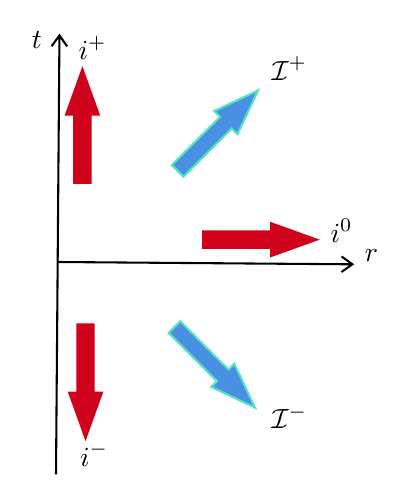
\begin{tikzpicture}[x=0.75pt,y=0.75pt,yscale=-0.75,xscale=0.75]
		%uncomment if require: \path (0,609); %set diagram left start at 0, and has height of 609
		
		%Shape: Axis 2D [id:dp7821872331367214] 
		\draw  (196.6,214.86) -- (385.94,216.34)(197.75,69.29) -- (195.53,351.32) (378.98,211.29) -- (385.94,216.34) -- (378.9,221.29) (192.69,76.25) -- (197.75,69.29) -- (202.69,76.33)  ;
		%Up Arrow [id:dp5623641448201375] 
		\draw  [color={rgb, 255:red, 208; green, 2; blue, 27 }  ,draw opacity=1 ][fill={rgb, 255:red, 208; green, 2; blue, 27 }  ,fill opacity=1 ] (202,120.2) -- (212.5,91) -- (223,120.2) -- (217.75,120.2) -- (217.75,164) -- (207.25,164) -- (207.25,120.2) -- cycle ;
		%Up Arrow [id:dp9355069637780506] 
		\draw  [color={rgb, 255:red, 208; green, 2; blue, 27 }  ,draw opacity=1 ][fill={rgb, 255:red, 208; green, 2; blue, 27 }  ,fill opacity=1 ] (225,298.8) -- (214.5,328) -- (204,298.8) -- (209.25,298.8) -- (209.25,255) -- (219.75,255) -- (219.75,298.8) -- cycle ;
		%Up Arrow [id:dp8020921103254861] 
		\draw  [color={rgb, 255:red, 208; green, 2; blue, 27 }  ,draw opacity=1 ][fill={rgb, 255:red, 208; green, 2; blue, 27 }  ,fill opacity=1 ] (333.8,190) -- (363,200.5) -- (333.8,211) -- (333.8,205.75) -- (290,205.75) -- (290,195.25) -- (333.8,195.25) -- cycle ;
		%Up Arrow [id:dp5136238103533108] 
		\draw  [color={rgb, 255:red, 80; green, 227; blue, 194 }  ,draw opacity=1 ][fill={rgb, 255:red, 74; green, 144; blue, 226 }  ,fill opacity=1 ] (297.24,117.91) -- (325.31,104.69) -- (312.09,132.76) -- (308.37,129.05) -- (277.4,160.02) -- (269.98,152.6) -- (300.95,121.63) -- cycle ;
		%Up Arrow [id:dp5383249274435937] 
		\draw  [color={rgb, 255:red, 80; green, 227; blue, 194 }  ,draw opacity=1 ][fill={rgb, 255:red, 74; green, 144; blue, 226 }  ,fill opacity=1 ] (310.09,280.24) -- (323.31,308.31) -- (295.24,295.09) -- (298.95,291.37) -- (267.98,260.4) -- (275.4,252.98) -- (306.37,283.95) -- cycle ;
		
		% Text Node
		\draw (332,81) node [anchor=north west][inner sep=0.75pt]   [align=left] {$\displaystyle \mathcal{I}^{+}$};
		% Text Node
		\draw (332,305) node [anchor=north west][inner sep=0.75pt]   [align=left] {$\displaystyle \mathcal{I}^{-}$};
		% Text Node
		\draw (208,68) node [anchor=north west][inner sep=0.75pt]   [align=left] {$\displaystyle i^{+}$};
		% Text Node
		\draw (209,329) node [anchor=north west][inner sep=0.75pt]   [align=left] {$\displaystyle i^{-}$};
		% Text Node
		\draw (178,65) node [anchor=north west][inner sep=0.75pt]   [align=left] {$\displaystyle t$};
		% Text Node
		\draw (370,185) node [anchor=north west][inner sep=0.75pt]   [align=left] {$\displaystyle i^{0}$};
		% Text Node
		\draw (392,205) node [anchor=north west][inner sep=0.75pt]   [align=left] {$\displaystyle r$};
	\end{tikzpicture}
\end{center}
\caption{共形无穷远定义}
\end{marginfigure}
\begin{itemize}
	\item[$i^+$]:类时未来无穷远,$r$一定,$t\to+\infty$;
	\item[$i^-$]:类时过去无穷远,$r$一定,$t\to-\infty$;
	\item[$i^0$]:类空无穷远,$t$一定,$r\to+\infty$;
	\item[$\mathcal{I}^+$]:类光未来无穷远,$u$一定,$r\to+\infty$;
	\item[$\mathcal{I}^-$]:类光过去无穷远,$v$一定,$r\to+\infty$;
\end{itemize}
这五个无穷远合称为\textbf{共形无穷远}。

但是无穷远还是一个靠想象的概念,无法在这样的图中表现出来,继续考虑坐标变换,变到所谓光锥坐标:
\begin{equation}
	U\equiv\arctan u ,\quad V\equiv\arctan v
\end{equation}
度规在光锥坐标下变为:
\begin{equation}
	ds^2=\frac{1}{4\cos^2U\cos^2V}\cdot\left(-4dUdV+\sin^2(V-U)d{\Omega_2}^2\right),\quad -\frac{\pi}{2}<U\leq V<\frac{\pi}{2}
\end{equation}
现在我们牺牲对距离的精确描述,考虑Weyl变换之后,丢掉共形因子后的度规:
\begin{equation}\label{eq:15.6}
	\tilde{ds}^2=-4dUdV+\sin^2(V-U)d{\Omega_2}^2
\end{equation}
这样消去了在$\pm\frac{\pi}{2}$处的坐标奇性,我们称之为\textbf{共形紧化}。可以证明\cite{blau},两个相差共形变换的度规具有如下性质:
\begin{itemize}
	\item[1.] 由于$\tilde{ds}^2\iff ds^2=0$,所以光锥不变,即时空因果结构不发生改变;
	\item[2.] 向量场的类时、类空和类光性质不变;
	\item[3.] 类时和类空曲线还是类时或者类空的,但是类时或者类空测地线不一定仍是测地线,但是类光测地线依然是类光测地线。
\end{itemize}
从这个意义上看,如果我们只关注时空的因果结构,完全可以考虑共形紧化之后的度规,重点是共形紧化后坐标变成有限区间内取值,这使得我们有希望在时空图上表现出共形无限远。继续对\ref{eq:15.6}做变换:
\begin{equation}
	T=U+V,\quad R=U-V,\overset{\Rightarrow}{\text{overall}}t\pm r=\tan\frac{1}{2}\left(T\pm R\right)
\end{equation}
度规变为:
\begin{equation}
	\tilde{ds}^2=-dT^2+dR^2+\sin^2Rd{\Omega_2}^2,\quad|T|+R<\pi,0\leq R<\pi
\end{equation}
最后一项角向不用在意\sn{坐标变换的时候我们只是把$r,t$进行变换,没有将他们与角向坐标混合},现在整个时空图是一个有限大小的图,其上面的每一点表示一个球面(除了$i^0$),而且共形无限远以边界的形式表现出来:
\begin{figure}[H]
	\centering
	\begin{tikzpicture}[scale=3.5]
		\message{Penrose diagram (radius r)^^J}
		
		\def\Nlines{4} % number of world lines (at constant r/t)
		\def\ta{tan(90*1.0/(\Nlines+1))} % constant r/t value 1
		\def\tb{tan(90*2.0/(\Nlines+1))} % constant r/t value 2
		\coordinate (O) at ( 0, 0); % center: origin (r,t) = (0,0)
		\coordinate (S) at ( 0,-1); % south: t=-infty, i-
		\coordinate (N) at ( 0, 1); % north: t=+infty, i+
		\coordinate (E) at ( 1, 0); % east:  r=+infty, i0
		\coordinate (X) at ({penroseu(\tb,\tb)},{penrosev(\tb,\tb)});
		\coordinate (X0) at ({penroseu(\ta,-\tb)},{penrosev(\ta,-\tb)});
		
		% AXES
		\fill[mylightblue] (N) -- (E) -- (S) -- cycle;
		\draw[->,thick] (-0.1,0) -- (1.2,0) node[below right=-2] {$R$};
		\draw[->,thick] (0,-1.1) -- (0,1.2) node[left=-1] {$T$};
		
		% INFINITY LABELS
		\node[above=1,above left=0,mydarkblue,align=center] at (O)
		{$r=0$};
		\node[left=6,above right=-2,mydarkblue,align=center] at (1,0.04)
		{spacelike\\[-2]infinity ($i^0$)\\[-2]$r=+\infty$};
		\node[above=6,below right=0,mydarkpurple,align=left] at (0.04,-1)
		{$t=-\infty$\\[-2]past timelike\\[-2]infinity ($i^-$)};
		\node[below=6,above right=0,mydarkpurple,align=left] at (0.04,1)
		{future timelike\\[-2]infinity ($i^+$)\\[-2]$t=+\infty$};
		\node[mydarkblue,above right,align=right] at (57:0.68)
		{future lightlike\\[-2]infinity ($\mathcal{I}^+$)};
		\node[mydarkblue,below right,align=right] at (-60:0.68)
		{past lightlike\\[-2]infinity ($\mathcal{I}^-$)};
		
		% CONE BACK
		\coneback{X};
		\coneback{X0};
		
		% WORLD LINES
		\draw[world line] (N) -- (S);
		\draw[world line] (O) -- (E);
		\message{Making world lines...^^J}
		\foreach \i [evaluate={\c=\i/(\Nlines+1); \ct=tan(90*\c);}] in {1,...,\Nlines}{
			\message{  Running i/N=\i/\Nlines, c=\c, tan(90*\c)=\ct...^^J}
			\draw[world line t,samples=\Nsamples,smooth,variable=\t,domain=0.001:1] % constant t
			plot(\t,{-penrose(\t*pi/2,\ct)})
			plot(\t,{ penrose(\t*pi/2,\ct)});
			\draw[world line,samples=\Nsamples,smooth,variable=\r,domain=-1:1] % constant r
			plot({penrose(\r*pi/2,\ct)},\r);
		}
		\draw[thick,mydarkblue] (N) -- (E) -- (S) -- cycle;
		
		% CONSTANT
		\draw[->,mydarkpurple!80!black,shorten <=0.4] % constant r
		(0.66,{-penrose(0.66*pi/2,tan(90*3/(\Nlines+1)))}) to[out=-70,in=150]++ (-45:0.23)
		node[right=-1] {$t=\text{constant}$};
		\draw[->,mydarkblue!80!black,shorten <=0.4] % constant t
		({penrose(-0.27*pi/2,tan(90*3/(\Nlines+1)))},-0.27) to[out=-55,in=170]++ (-35:0.3)
		node[right=-1] {$r=\text{constant}$};
		
		% PARTICLE
		\draw[particle,decoration={markings,mark=at position 0.24 with {\arrow{latex}},
			mark=at position 0.55 with {\arrow{latex}},
			mark=at position 0.82 with {\arrow{latex}}},postaction={decorate}]
		(S) to[out=90,in=-80] (X0) to[out=100,in=-95] (X) to[out=85,in=-90] (N);
		
		% LIGHT CONE FRONT
		\conefront{X};
		\conefront{X0};
		
		% PHOTON
		\draw[->,photon] (O) -- (0.5,0.5) node[above=2,right=1] {photon};
		
		% TICKS
		\tick{E}{90} node[right=4,below=-1] {$+\pi$};
		\tick{S}{ 0} node[left=-1] {$-\pi$};
		\tick{N}{ 0} node[left=-1] {$+\pi$};
	\end{tikzpicture}
	\caption{Minkowski时空彭罗斯图}
\end{figure}
这种类光测地线都是$45^\circ$斜线,而且能表示共形无限远的图称为彭罗斯图。这个图还有另一种更常用的画法,其实是比上面的形式多出一个维度,用图上左右部分两个点表示一个球$\mathcal{S}^2$,表示球上的一对对径点。原先在上图中只能画成折线的测地线现在可以展开画为曲线:
\begin{figure}[H]
	\centering
	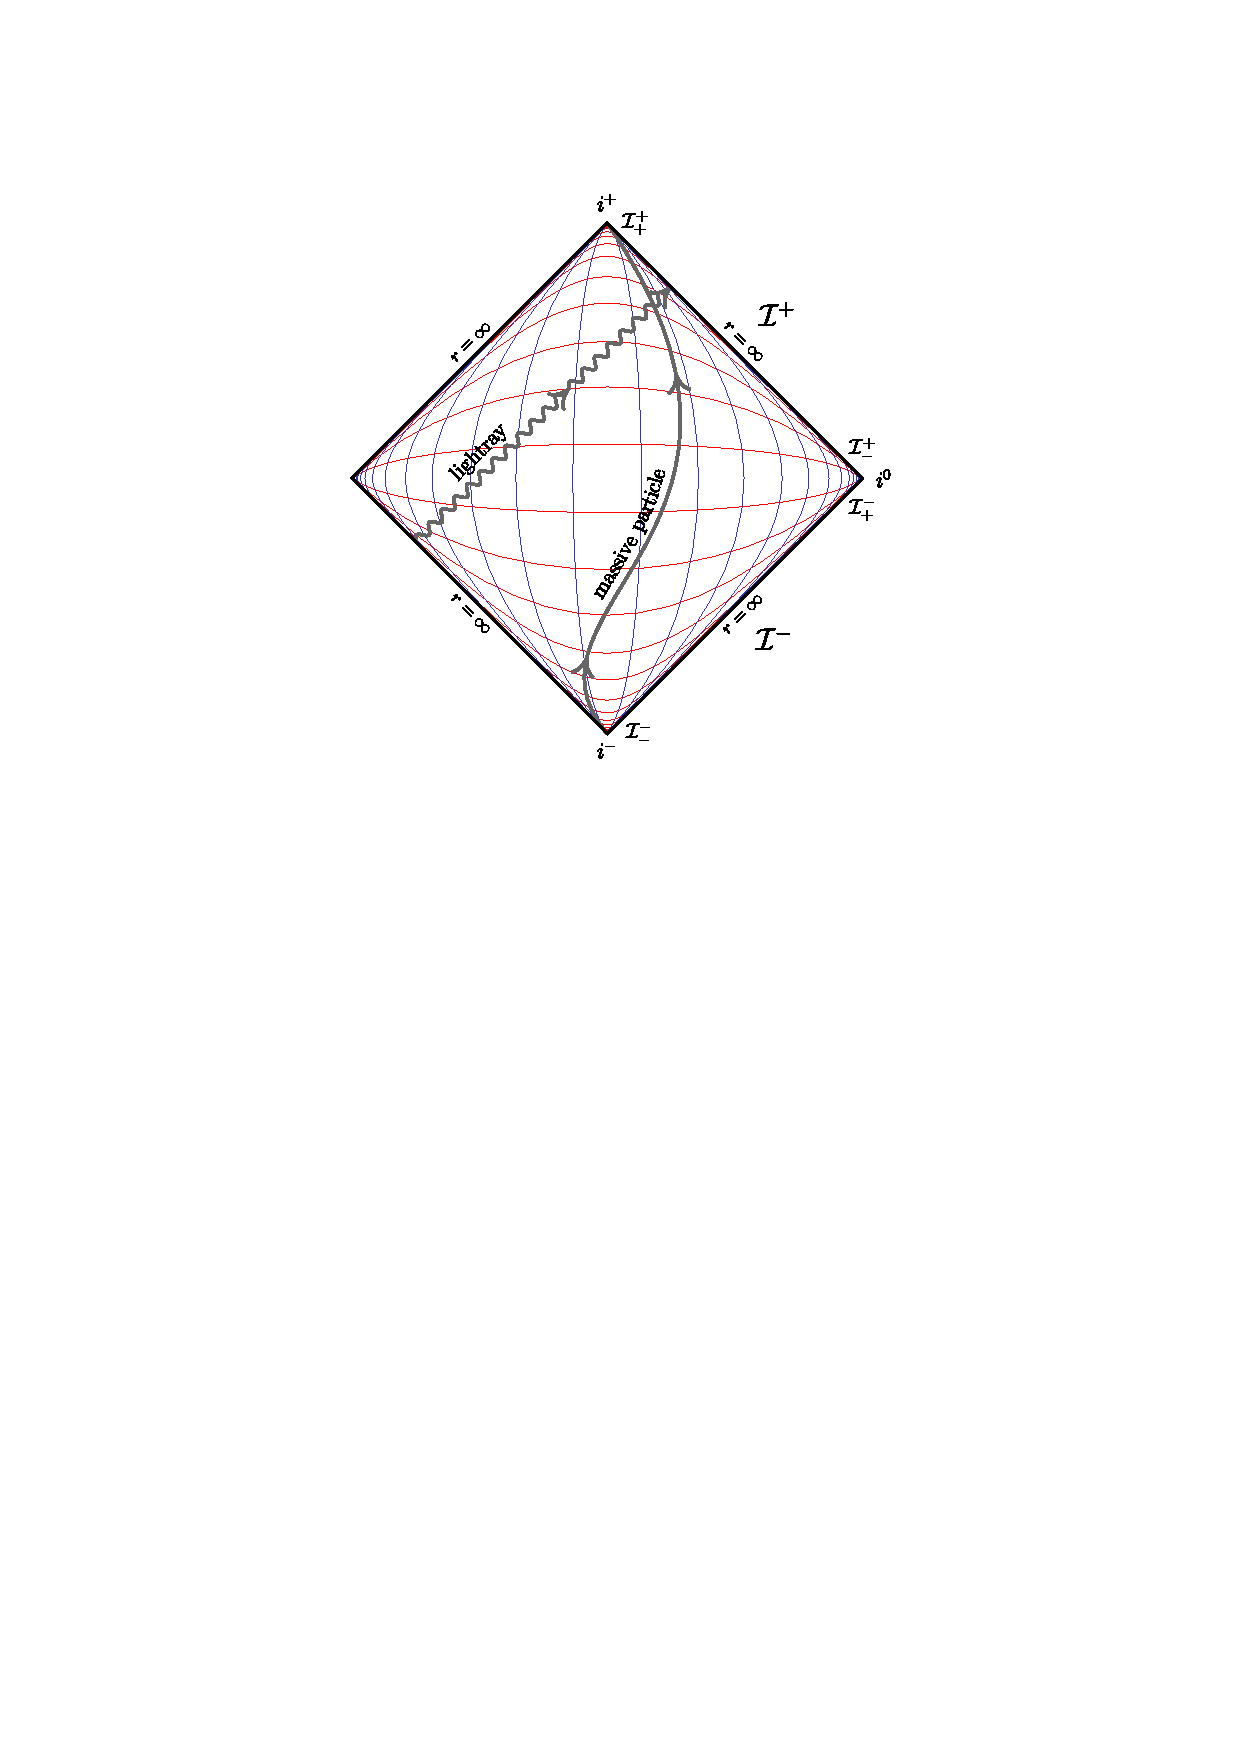
\includegraphics[width=0.618\linewidth]{figs/cover.pdf}
	\caption{Minkowski时空彭罗斯图的另一种形式}
\end{figure}

注意前面的几个Penrose图都特别对$i^+,\mathcal{I}_+^+;i^-,\mathcal{I}_-^-$以及$i^0,\mathcal{I}_+^-,\mathcal{I}_-^+$后面我们将会看到,场在这几个点上其实是多值的,或者说极限与趋近方向有关,所以必须进行区分,这几个点并不是一个点,即使是极限的意义下也不是!

在我们考虑的散射过程中,有质量粒子总是从$i^-$出发,通过类时测地线最终抵达$i^+$,而无质量粒子总是从$\mathcal{I}_-$出发走$45^\circ$斜线到达$\mathcal{I}_+$。


\section{Celestial Sphere}
\begin{figure}[htbp]
	\centering
	\tikzset{every picture/.style={line width=0.75pt}} %set default line width to 0.75pt        
	
	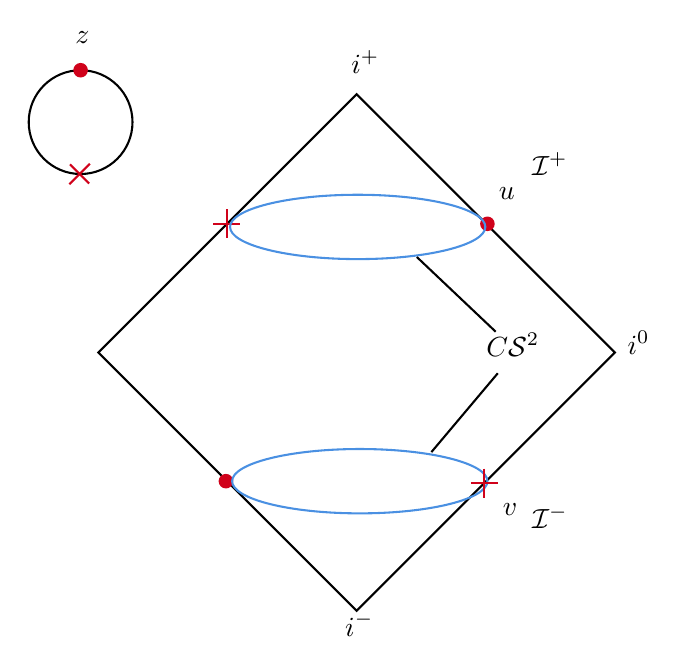
\begin{tikzpicture}[x=0.75pt,y=0.75pt,yscale=-1,xscale=1]
		%uncomment if require: \path (0,609); %set diagram left start at 0, and has height of 609
		
		%Shape: Square [id:dp4061795534153141] 
		\draw   (281,97.55) -- (405.45,222) -- (281,346.45) -- (156.55,222) -- cycle ;
		%Shape: Circle [id:dp08927835248745741] 
		\draw   (123,111) .. controls (123,97.19) and (134.19,86) .. (148,86) .. controls (161.81,86) and (173,97.19) .. (173,111) .. controls (173,124.81) and (161.81,136) .. (148,136) .. controls (134.19,136) and (123,124.81) .. (123,111) -- cycle ;
		\draw  [color={rgb, 255:red, 208; green, 2; blue, 27 }  ,draw opacity=1 ] (212,160) -- (225,160)(218.5,153) -- (218.5,167) ;
		\draw  [color={rgb, 255:red, 208; green, 2; blue, 27 }  ,draw opacity=1 ] (142.9,131.4) -- (152.1,140.6)(152.45,131.05) -- (142.55,140.95) ;
		%Shape: Circle [id:dp8549954932536064] 
		\draw  [color={rgb, 255:red, 208; green, 2; blue, 27 }  ,draw opacity=1 ][fill={rgb, 255:red, 208; green, 2; blue, 27 }  ,fill opacity=1 ] (145,86) .. controls (145,84.34) and (146.34,83) .. (148,83) .. controls (149.66,83) and (151,84.34) .. (151,86) .. controls (151,87.66) and (149.66,89) .. (148,89) .. controls (146.34,89) and (145,87.66) .. (145,86) -- cycle ;
		%Shape: Circle [id:dp26121264153734547] 
		\draw  [color={rgb, 255:red, 208; green, 2; blue, 27 }  ,draw opacity=1 ][fill={rgb, 255:red, 208; green, 2; blue, 27 }  ,fill opacity=1 ] (341,160) .. controls (341,158.34) and (342.34,157) .. (344,157) .. controls (345.66,157) and (347,158.34) .. (347,160) .. controls (347,161.66) and (345.66,163) .. (344,163) .. controls (342.34,163) and (341,161.66) .. (341,160) -- cycle ;
		%Shape: Ellipse [id:dp2797557616828865] 
		\draw  [color={rgb, 255:red, 74; green, 144; blue, 226 }  ,draw opacity=1 ] (220,161.5) .. controls (220,152.94) and (247.53,146) .. (281.5,146) .. controls (315.47,146) and (343,152.94) .. (343,161.5) .. controls (343,170.06) and (315.47,177) .. (281.5,177) .. controls (247.53,177) and (220,170.06) .. (220,161.5) -- cycle ;
		%Shape: Circle [id:dp422435135864375] 
		\draw  [color={rgb, 255:red, 208; green, 2; blue, 27 }  ,draw opacity=1 ][fill={rgb, 255:red, 208; green, 2; blue, 27 }  ,fill opacity=1 ] (215,284) .. controls (215,282.34) and (216.34,281) .. (218,281) .. controls (219.66,281) and (221,282.34) .. (221,284) .. controls (221,285.66) and (219.66,287) .. (218,287) .. controls (216.34,287) and (215,285.66) .. (215,284) -- cycle ;
		%Shape: Ellipse [id:dp2997647396682279] 
		\draw  [color={rgb, 255:red, 74; green, 144; blue, 226 }  ,draw opacity=1 ] (221,284) .. controls (221,275.44) and (248.53,268.5) .. (282.5,268.5) .. controls (316.47,268.5) and (344,275.44) .. (344,284) .. controls (344,292.56) and (316.47,299.5) .. (282.5,299.5) .. controls (248.53,299.5) and (221,292.56) .. (221,284) -- cycle ;
		\draw  [color={rgb, 255:red, 208; green, 2; blue, 27 }  ,draw opacity=1 ] (336,285) -- (349,285)(342.5,278) -- (342.5,292) ;
		%Straight Lines [id:da40913177395617817] 
		\draw    (310,176) -- (348,212) ;
		%Straight Lines [id:da5756898592429918] 
		\draw    (349,232) -- (317,270) ;
		
		% Text Node
		\draw (144,66) node [anchor=north west][inner sep=0.75pt]   [align=left] {$\displaystyle z$};
		% Text Node
		\draw (348,141) node [anchor=north west][inner sep=0.75pt]   [align=left] {$\displaystyle u$};
		% Text Node
		\draw[yshift=1em] (350,280) node [anchor=north west][inner sep=0.75pt]   [align=left] {$\displaystyle v$};
		% Text Node
		\draw (342,211) node [anchor=north west][inner sep=0.75pt]   [align=left] {$\displaystyle C\mathcal{S}^{2}$};
		% Text Node
		\draw (274,346) node [anchor=north west][inner sep=0.75pt]   [align=left] {$\displaystyle i^{-}$};
		% Text Node
		\draw (277,75) node [anchor=north west][inner sep=0.75pt]   [align=left] {$\displaystyle i^{+}$};
		% Text Node
		\draw (364,124) node [anchor=north west][inner sep=0.75pt]   [align=left] {$\displaystyle \mathcal{I}^{+}$};
		% Text Node
		\draw (364,294) node [anchor=north west][inner sep=0.75pt]   [align=left] {$\displaystyle \mathcal{I}^{-}$};
		% Text Node
		\draw (410,210) node [anchor=north west][inner sep=0.75pt]   [align=left] {$\displaystyle i^{0}$};
	\end{tikzpicture}
	\caption{Bondi坐标与天球}
	\label{fig:4}
\end{figure}
如图\ref{fig:4}所示,$\mathcal{I}^{\pm}$上的每一个点代表一个球面\sn{在这个图上是左右两边各一个点组成的对径点连成的圆周表示一个球面},我们称之为\text{天球}$C\mathcal{S}^2$,在SR的语境下,天球一般指观察者所看到的无限远区域,所以特指$\mathcal{I}^-$上的天球。

在类光无穷远处可以选取Bondi坐标来参数化天球,在$\mathcal{I}^+$上我们选取$(u,r,z,\bar z)$,其中$r\to \infty$,$(z,\bar z)$是球极投影到复平面来表示天球的角向坐标,这套坐标与$\{x^\mu\}$之间的关系为:
\begin{equation}
	x^\mu=\left(u+r,r\frac{z+\bar z}{1+z\bar z},ir\frac{\bar z-z}{1+z\bar z},r\frac{1-z\bar z}{1+z\bar z}\right)		
\end{equation}

在$\mathcal{I}^-$上我们选取$(v,r,z,\bar z)$,其中$r\to \infty$,注意现在角向坐标和$\mathcal{I}^+$上的选取是对径认同的关系,也就是说$z\mapsto-\frac{1}{\bar z}$:
\begin{equation}
	x^\mu=\left(v-r,-r\frac{z+\bar z}{1+z\bar z},-ir\frac{\bar z-z}{1+z\bar z},-r\frac{1-z\bar z}{1+z\bar z}\right)		
\end{equation}
从上面的式子也可看出$\mathcal{I}^\pm$上两套坐标空间部分的关系的确为空间反演,在图\ref{fig:4}中我们也通过{\color{red}$\bullet$}和{\color{red}$\times$}标记出来了。
\begin{figure}[htbp]
	\centering
	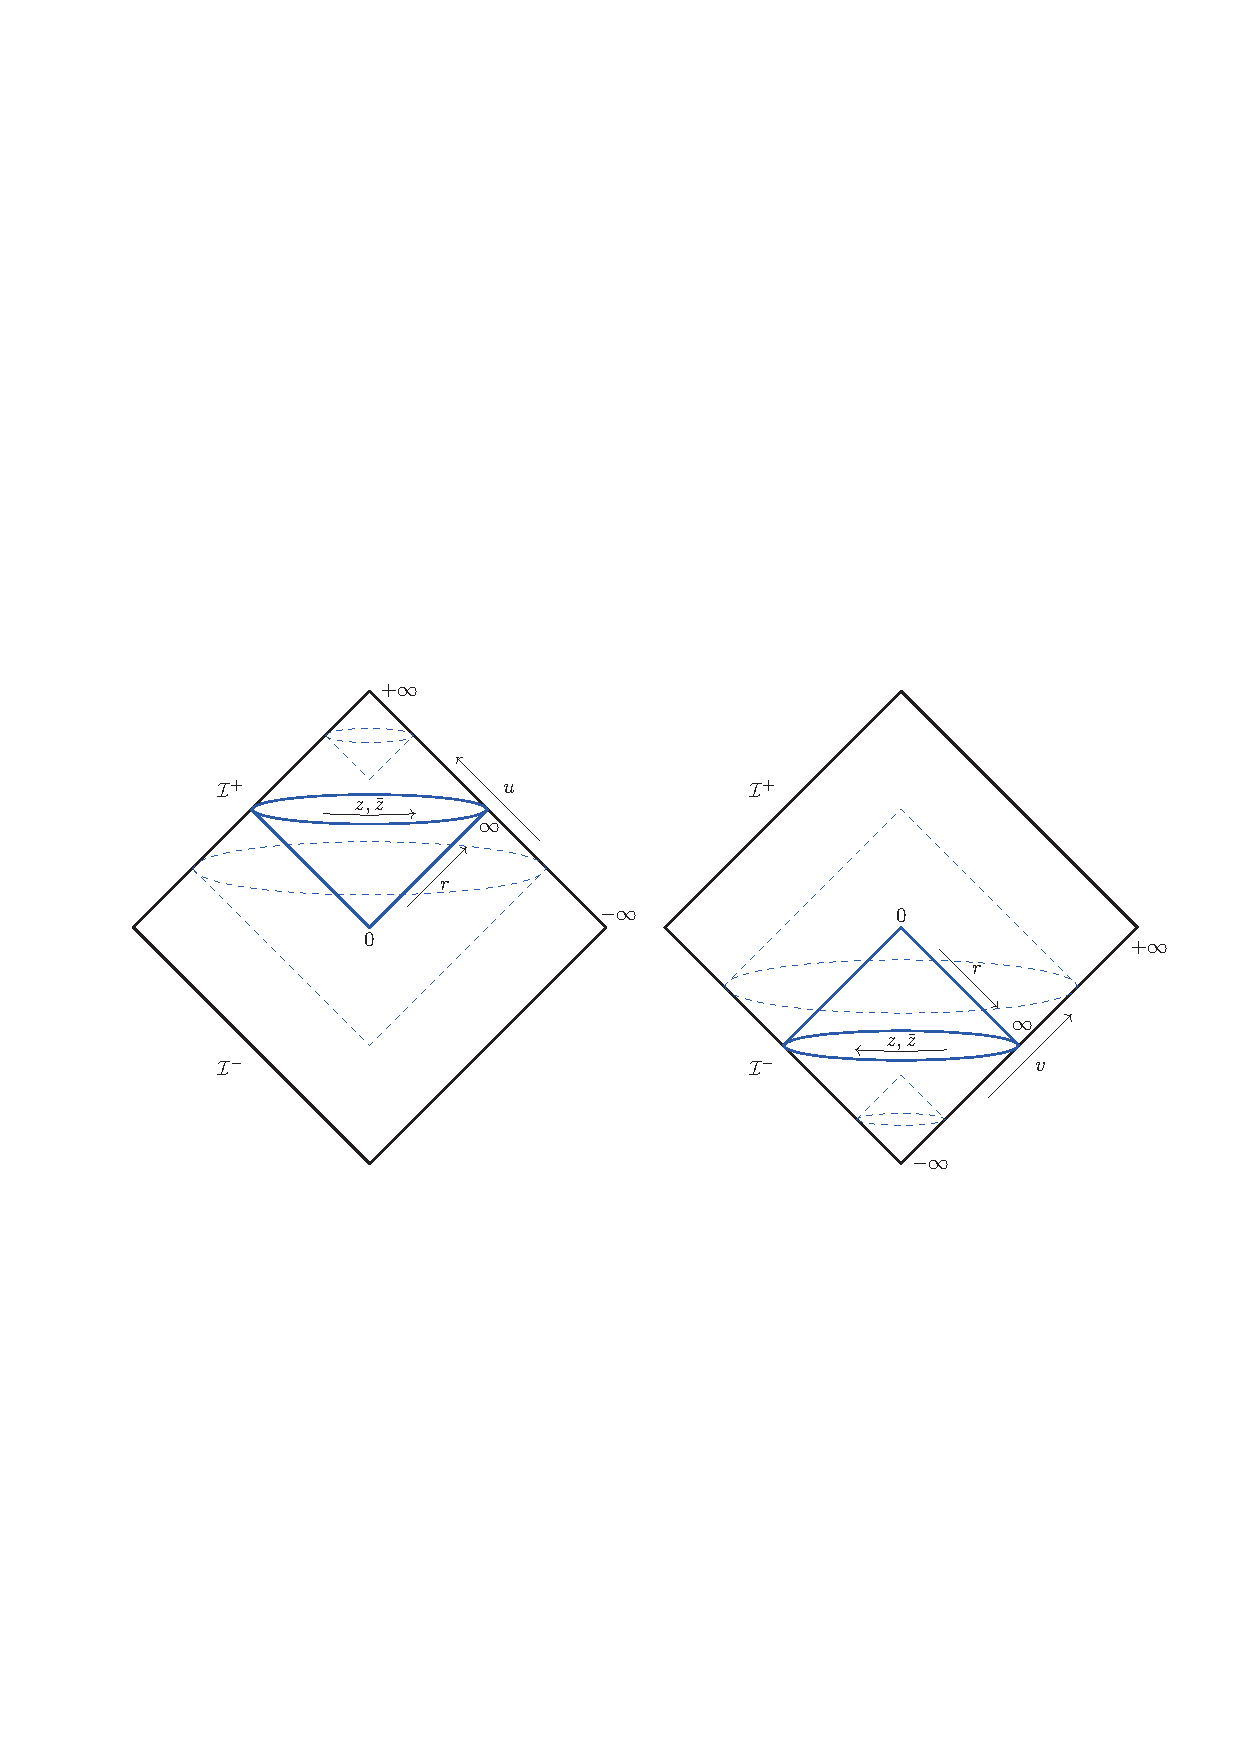
\includegraphics[width=\linewidth]{figs/fig1.pdf}
	\caption{Bondi坐标}
\end{figure}

现在考虑Lorentz变换对天球的作用,也就是要考虑Lorentz变换下Bondi坐标在$r\to\infty$怎么变。我们以$\mathcal{I}^+$上的天球为例,首先考虑$r$的变化。思路就是根据$r=\sqrt{x^ix_i}$,$x^\mu\mapsto{\Lambda^\mu}_{\nu}x^\nu$以及$SO(3,1)^\uparrow\cong SL(2,\mathbb{C})/\mathbb{Z}_2$导致的\ref{eq:8.1}进行计算,并取$r\to\infty$的极限,经过冗长的计算后得到\sn{本节的详细计算参考\cite{Oblak:2015qia}}:
\begin{equation}
	r'=r\cdot\frac{|az+b|^2+|cz+d|^2}{1+z\bar z}+\mathcal{O}(1)\equiv r\cdot F(z,\bar z)+\mathcal{O}(1)
\end{equation}
所以Lorentz变换下确实会把$r=\infty\mapsto r=\infty$。$u$的变换计算相对简单,注意到
\[t^2-r^2=u^2+2ur\]
式子左边是个Lorentz不变量,现在考虑的是某个固定$u$时的天球变换,所以$r\to\infty$后说明$2ur$是个Lorentz标量,代入$r$变换关系得到:
\begin{equation}
	u'=\frac{u}{F(z,\bar z)}+\mathcal{O}\left(\frac{1}{r}\right)
\end{equation}
注意,这里说明在一般的Lorentz变换后天球并非还是天球,因为$u$的变换依赖于角向坐标。如果现在只关心天球的角向坐标怎么变,不关心变换后每个点是属于哪一“时刻”的天球,计算后发现:
\begin{equation}
	z'=\frac{az+b}{cz+d}+\mathcal{O}\left(\frac{1}{r}\right)
\end{equation}
也就是说天球角向的变换就是$C\mathcal{S}^2$上的全局共形变换!但是写出这个形式我们利用了\ref{eq:8.1},这也就是前面为何要取$\tau_1=-\sigma_1$原因,本质上就是为了让这列公式形式更加漂亮,选取$\sigma_1$也不影响变换还是一个全局共形变换。天球在Lorentz变换下的变换可以用下图总结\sn{不少精美的插图都是直接取自\cite{Strominger:2017zoo}}:
\begin{figure}[htbp]
	\centering
	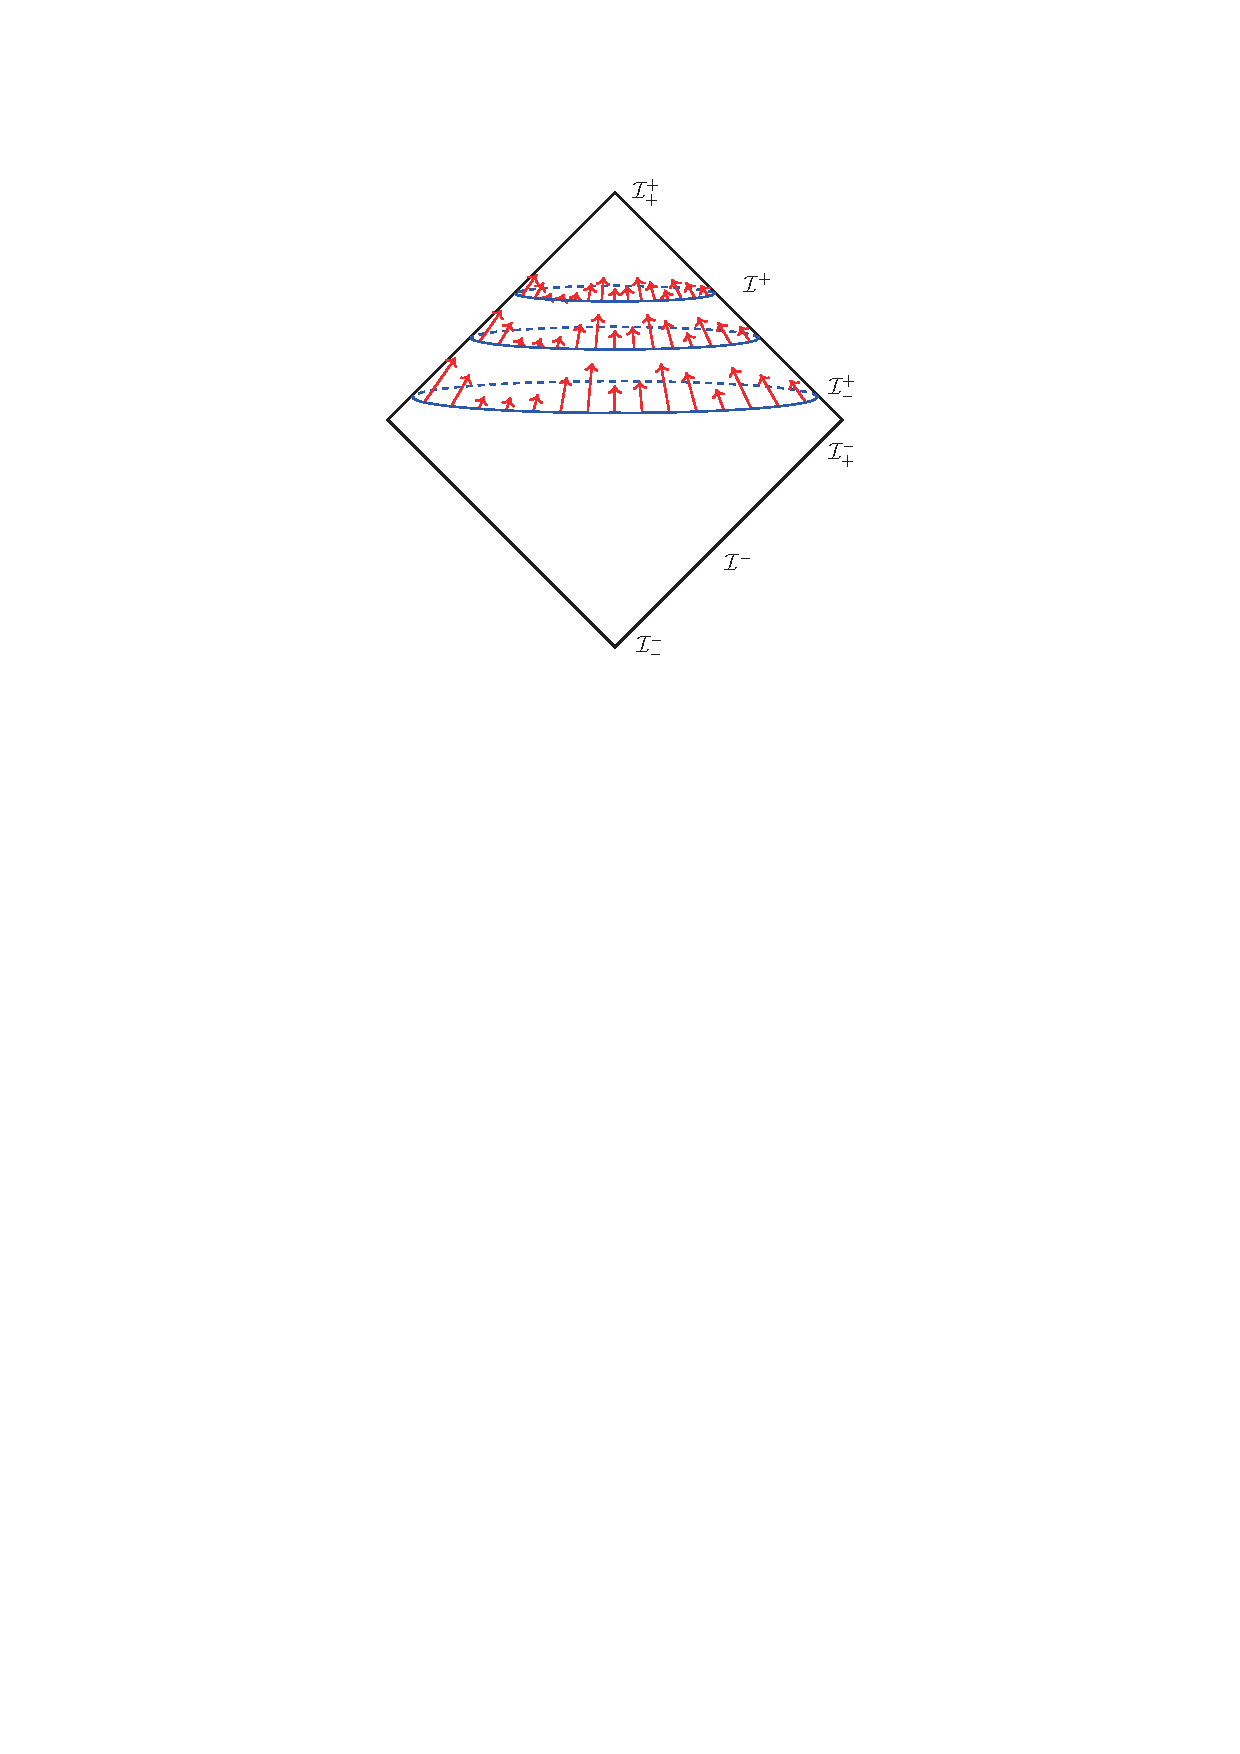
\includegraphics{figs/fig2.pdf}
	\caption{天球上的Lorentz变换}
\end{figure}

\section{Asymptotic flat spacetime: basic concepts}
所谓渐近平直时空简单点说就是在共形无限远处与Minkowski时空一致,渐近效应足够小允许存在引力波等解,但又要足够大能够排除无穷大能量这些非物理解。这一要求实际上可以用严格的与坐标无关的流形语言来描述\cite{lcb2}。这里考虑使用某一特定坐标系——Bondi坐标——的语言来进行阐述\cite{Compere:2019qed,Strominger:2017zoo},由于$\mathcal{I}^\pm$的处理方法类似,所以重点考虑于$\mathcal{I}^+$。

由于广义相对论是一个与坐标无关的理论,即理论本身具有微分同胚不变性,这是理论本身的冗余自由度,我们这里实际上是在对理论选取一个特定规范后进行描述。Bondi规范是最早也最自然的提法,当然也有其它规范选取\cite{Campiglia:2015kxa,Campiglia:2015lxa}。对于某个固定的$u(x^\mu)$,在时空上决定了一个超曲面,其上法矢为$n^\mu=g^{\mu\nu}\partial_\nu u$,第一个规范条件是要求这个超曲面类光\sn{关于超曲面的严格定义以及相关概念可参考\cite{lcb}},也就是说$n^\mu n_\mu=0\Rightarrow g^{uu}=0$;再定义$x^A,A=\{1,2\}$为角向坐标,与超曲面法矢相正交,即$\nabla_n x^A=n^\mu\partial_\mu x^A=0\Rightarrow g^{uA}=0$;最后一个要求是$r$取为\textbf{luminosity distance},这要求$\partial_r \det (g_{AB}/r^2)=0$。则$x^\mu=(u,r,x^A)$构成Bondi规范,上面的条件也等价于:
\begin{equation}
	g_{rr}=g_{rA}=0,\quad \partial_r\det\frac{g_{AB}}{r^2}=0
\end{equation}
在这个规范下,最一般的度规可以写作:\sn{后面若无特殊说明,对角向指标$A,B$求和}
\begin{equation}
	ds^2=g_{uu}du^2+2g_{ur}dudr+2g_{uA}dudx^A+g_{AB}dx^Adx^B
\end{equation}
对于Minkowski时空,Bondi guage就是选取retarded coordinate,$u=t-r$,度规形式为:
\begin{equation}
	ds^2=-du^2-2dudr+r^2\gamma_{AB}dx^Adx^B
\end{equation}
渐近平直即要求$r\to\infty$时,时空度规与上面一致。Bondi等人计算后对渐近平直时空的度规在$r\to\infty$的渐近行为给予了如下限制\cite{Bondi:1962px,Sachs:1962wk}:
\begin{equation}\label{eq:17.4}
	\begin{aligned}
		ds^2=&-du^2-2dudr+r^2\gamma_{AB}dx^Adx^B\\
		&+\frac{2m_B}{r}du^2+rC_{AB}dx^Adx^B+D^B C_{AB}dudx^A\\
		&+\frac{1}{16r^2}C_{AB}C^{AB}dudr+\frac{1}{r}\left[\frac{4}{3}\left(N_A+u\partial_Am_B\right)-\frac{1}{8}\partial_A\left(C_{BC}C^{BC}\right)\right]dudx^A\\
		&+\frac{1}{4}\gamma_{AB}C_{CD}C^{CD}dx^Adx^B+\cdots
	\end{aligned}
\end{equation}
其中$\gamma^{AB}C_{AB}=0,C_{AB}=C_{BA}$,角向指标使用$\gamma^{AB}$进行升降,而$D^A$是与$\gamma^{AB}$适配的协变导数\footnote{对于任何一个流形,给定度规后都唯一存在一个无挠的联络$\nabla$使得$\nabla_X g=0,\forall X\in\mathscr{X}(\mathcal{M})$,称为Levi-Civita联络,对应的Clifford符号$\nabla_{e_\mu}e_\nu=\Gamma_{\mu\nu}^{\lambda}e_\lambda$由下式给出:
\[\Gamma^\lambda_{\mu\nu}=\frac{1}{2}g^{\lambda\sigma}\left(\partial_\mu g_{\nu\sigma}+\partial_\nu g_{\mu\sigma}-\partial_\sigma g_{\mu\nu}\right)\]}。这里特别注意$u,r$并不是Minkowski中的retarded coordinates!只是在$r\to\infty$时$u\approx \tilde t-\tilde r$\sn{这里的$\tilde t,\tilde r$是指Minkowski时空中的通常四维坐标,也就是使得度规为$\eta_{\mu\nu}$的坐标}。同时还要求物质能动张量满足:
\begin{align*}
	T^M_{uu}\sim\mathcal{O}(r^{-2}),& &T^M_{ur}\sim\mathcal{O}(r^{-4}),&&T^M_{rr}\sim\mathcal{O}(r^{-4})\\
	T^M_{uA}\sim\mathcal{O}(r^{-2}),&&T^M_{rA}\sim\mathcal{O}(r^{-3}),&&T^M_{AB}\sim\mathcal{O}(r^{-1})
\end{align*}
而且由于是在$\mathcal{I}^+$上考虑问题,所以这些能动张量都来源于无质量粒子。

\ref{eq:17.4}引进的这些参数都是有具体的物理意义的:
\begin{itemize}
	\item[$\bullet$]$m_B$:\textbf{Bondi mass aspect},物理意义是在$\mathcal{I}^+$的$u$处天球上观察得到的时空的能量角密度分布。\textbf{Bondi mass}可以通过积分$M(u)=\oint_{\mathcal{S}^2_\infty}\mathrm{d}^2\Omega m_B(u,x^A)$给出,$u\to-\infty$时,Bondi mass等于ADM能量。
	\item[$\bullet$]$C_{AB}$:这个量根据无迹对称约束,会给出两种极化模式(或者说引力子的两个螺旋度取值),它完全确定了$\mathcal{I}^+$上的引力波辐射,根据他可以定义\textbf{Bondi news tensor}$N_{AB}=\partial_u C_{AB}$,这个量可以和电磁Fraday张量$F_{uz}=\partial_u A_z$\sn{后面章节将会看到为何是这个形式}类比,它的平方正比于$\mathcal{I}^+$上的能流。
	\item[$\bullet$]$N_A$:\textbf{angular momentum aspect},这是相对于$r=0$这一点的角动量角密度分布,对他在$\mathcal{S}^2_\infty$上积分得到在$\mathcal{I}^+$的$u$处天球上观察得到的时空的总角动量。
\end{itemize}

现在我们选取角向坐标为$x^A=(z,\bar z)$来简化讨论,更一般的讨论见\cite{Compere:2019qed}。这导致$\gamma_{AB}$对角项为0,由$C_{AB}$的无迹对称性质有$C_{zz}^C^{zz}=C_{\bar z\bar z}C^{\bar z\bar z}$,实际上这个条件可以强化为$(C_{zz})^*=C_{\bar z\bar z}$,后面的公式中下标$z\mapsto \bar z$只需要通过求复共轭即可。在这样的角向坐标选取下,\ref{eq:17.4}简化为\sn{注意到这里忽略了$r^{-2}dudr$贡献,而且相比于$r^2dzd\bar z$忽略了\ref{eq:17.4}最后一项$\mathcal{O}(1)$的贡献}:
\begin{equation}\label{eq:17.5}
	\begin{aligned}
		ds^2=&-du^2-2dudr+2r^2\gamma_{z\bar z}dzd{\bar z}\\
		&+\frac{2m_B}{r}du^2+rC_{zz}dz^2+rC_{\bar z\bar z}d{\bar z}^2+D^z C_{zz}dudz+D^{\bar z}C_{\bar z\bar z}dud\bar z\\
		&+\frac{1}{r}\left[\frac{4}{3}\left(N_A+u\partial_zm_B\right)-\frac{1}{4}\partial_z\left(C_{zz}C^{zz}\right)\right]dudz+c.c.+\cdots
	\end{aligned}
\end{equation}
其中$C_zz,N_z,m_B$按照\ref{eq:17.4}类似定义,而且只与$(u,z,\bar z)$有关,与$r$无关。所以渐近平直时空的度规渐近式(在Bondi gauge下)可以概括为:
\begin{align*}
	&g_{uu}=-1+\mathcal{O}(r^{-1}),&&g_{ur}=-1+\mathcal{O}(r^{-2}),&&g_{uz}=\mathcal{O}(1)\\
	&g_{zzz}=\mathcal{O}(1),&&g_{z\bar z}=r^2\gamma_{z\bar z}+\mathcal{O}(1),&&g_{rr}=g_{rz}=0
\end{align*}
在不少文献中\cite{Pasterski:2021rjz,Kapec:2014opa,Raclariu:2021zjz}也经常见到\ref{eq:17.5}的另一种等价写法\sn{等价性并不显然,实际上,说他们等价,并不是说可以直接通过\ref{eq:17.5}得到\ref{eq:17.6},而是\ref{eq:17.6}形势下参量由场方程诱导的约束条件的形式会与\ref{eq:17.5}中的不同,他们的等价性隐藏在约束条件之中了。}:
\begin{equation}\label{eq:17.6}
	\begin{aligned}
		ds^2=&-du^2-2dudr+2r^2\gamma_{z\bar z}dzd{\bar z}\\
		&+\frac{2m_B}{r}du^2+rC_{zz}dz^2+rC_{\bar z\bar z}d{\bar z}^2+2g_{uz}dudz+2g_{u\bar z}dud\bar z+\cdots
	\end{aligned}
\end{equation}
其中:
\begin{equation}
	g_{uz}=\frac{1}{2}D^zC_{zz}+\frac{1}{6r}C_{zz}D_zC^{zz}+\frac{2}{3r}N_z+\mathcal{O}(r^{-2})
\end{equation}
不过这些对度规的限制都只是纯粹的几何意义上的,度规还必须是爱因斯坦场方程的解\sn{不少文献直接选取单位为$c=\hbar=8\pi G=1$,但是这样做实际上消去了所有量纲,无法再使用量纲分析这一工具\cite{Tong}。}:
\begin{equation}
	R_{\mu\nu}-\frac{1}{2}g_{\mu\nu}R=8\pi G T^M_{\mu\nu}
\end{equation}
\begin{remark}
	这里我们讨论一下前面对度规的约束为何是纯几何的,以\ref{eq:17.5}为例,我们计算$dudz$这一项的系数,我们先暂且设为$U_z$,根据Weyl张量的定义:
	\begin{equation}
		C_{\mu\nu\rho\sigma}=R_{\mu\nu\rho\sigma}+\frac{1}{2}\left(g_{\nu\rho}R_{\sigma\mu}+g_{\mu\sigma}R_{\rho\nu}-g_{\nu\sigma}R_{\rho\mu}-g_{\mu\rho}R_{\sigma\nu}\right)+\frac{1}{6}R\left(g_{\mu\rho}g_{\sigma\nu}-g_{\mu\sigma}g_{\rho\nu}\right)
	\end{equation}
	我们感兴趣的是下面两个分量:
	\begin{equation}
		C_{rzzrz}=R_{rzrz}-\frac{1}{2}g_{zz}R_{rr},\quad C_{rurz}=R_{rurz}+\frac{1}{2}(g_{ur}R_{rz}-g_{uz}R_{rr})
	\end{equation}
	代入$ds^2$一通计算猛如虎:
	\begin{equation}
		C_{rzzrz}=\mathcal{O}(r^{-3}),\quad C_{rurz}=-\frac{1}{4r^2}\left(U_z-D^z C_{zz}\right)+\mathcal{O}(r^{-3})
	\end{equation}
	显然,为了满足渐近平直性,要求$U_z=D^zC_{zz}$,推导过程中我们完全没有使用场方程。
\end{remark}
使用\ref{eq:17.6}的约定,利用场方程代入度规进行计算,逐项比较得到三个量满足的约束条件为:
\begin{equation}
	\begin{aligned}
		\partial_u m_B=&\frac{1}{4}D_z^2N^{zz}+\frac{1}{4}D_{\bar z}^2N^{\bar z\bar z}-\frac{1}{2}T^M_{uu}-\frac{1}{4}N_{zz}N^{zz}\\
		\partial_u N_z=&-\frac{1}{4}\left(D_zD_{\bar z}^2C^{\bar z\bar z}-D^3_zC^{zz}\right)-T^{M}_{uz}+\partial_z m_B+\frac{1}{16}D_zz\partial_u(C_{zz}C^{zz})\\
		&-\frac{1}{4}N^{zz}D_zC_{zz}-\frac{1}{4}N_{zz}D_zC^{zz}-\frac{1}{4}D_z\left(C^{zz}N_{zz}-N^{zz}C_{zz}\right)
	\end{aligned}
\end{equation}
其中
\begin{equation}
	T_{\mu\nu}(u,z,\bar z)=8\pi G\lim_{r\to\infty}r^2 T^M_{\mu\nu}(u,z,\bar z)
\end{equation}

对$\mathcal{I}^{-}$可以类似分析,这里仅罗列结果\sn{这里$r\to\infty,v\approx t+r$,角向坐标与$\mathcal{I}^{+}$上的对径认同}:
\begin{equation}
	\begin{aligned}
		ds^2=&-dv^2+2dvdr+2r^2\gamma_{z\bar z}dzd{\bar z}\\
		&+\frac{2m^-_B}{r}dv^2+rD_{zz}dz^2+rD_{\bar z\bar z}d{\bar z}^2+2g_{vz}dvdz+2g_{v\bar z}dvd\bar z+\cdots
	\end{aligned}
\end{equation}
其中\sn{这里$D^{AB}$相当于前面的$C^{AB}$,不要与协变导数弄混!}
\begin{equation}
	g_{vz}=-\frac{1}{2}D^zD_{zz}-\frac{1}{6r}D_{zz}D_zD^{zz}-\frac{2}{3r}N^-_z+\mathcal{O}(r^{-2})
\end{equation}
类似的可以定义News tensor:
\begin{equation}
	M_{zz}\equiv \partial_v D_{zz}
\end{equation}
约束条件为:
\begin{equation}
	\begin{aligned}
		\partial_u m^-_B=&\frac{1}{4}D_z^2M^{zz}+\frac{1}{4}D_{\bar z}^2M^{\bar z\bar z}+\frac{1}{2}T^M_{vv}+\frac{1}{4}M_{zz}M^{zz}\\
		\partial_u N^-_z=&\frac{1}{4}\left(D_zD_{\bar z}^2D^{\bar z\bar z}-D^3zD^{zz}\right)-T^{M}_{vz}-\partial_z m^-_B+\frac{1}{16}D_zz\partial_v(C_{zz}C^{zz})\\
		&-\frac{1}{4}M^{zz}D_zD_{zz}-\frac{1}{4}M_{zz}D_zD^{zz}-\frac{1}{4}D_z\left(D^{zz}M_{zz}-M^{zz}D_{zz}\right)
	\end{aligned}
\end{equation}

渐近平直时空也可以从时空图上一窥其特征\cite{zhaoliu},只要是渐近平直时空,Penrose图在$\mathcal{I}^\pm$边界上都类似于Minkowski时空图的直角形状。

\section{Asymptotic flat spacetime: BMS group}
\section{Asymptotic flat spacetime: charges}